%-----------------------------------------------------------------------------%
\chapter{\babTiga}
%-----------------------------------------------------------------------------%

Penelitian ini dibagi menjadi empat tahap: (1) Mendapatkan data microarray dan pengolahan awal; (2) Perancangan algoritma; (3) Melakukan eksperimen untuk mendapatkan \textit{hyperparameter} yang optimal. Kemudian dilanjutkan dengan  testing dan evaluasi. Gambaran umum dari penelitian ini seperti pada gambar bagan 1

\todo { untuk sementara copy paste dari laporan}

%-----------------------------------------------------------------------------%
\section{Gambaran Umum Penelitian}
%-----------------------------------------------------------------------------%

\todo { 1. include grafik \\
2. Bagian unsupervised dan supervised \\
3. RBM \\
4. Cost Function \\
5. DBN \\
6. Proses Multistep ranking \\
7. copy paste gambar tensorflow \\
8. list semua rumus yang dibutuhkan \\
9. tulis bab 2 yang isinya deep learning tutorial \\
 }
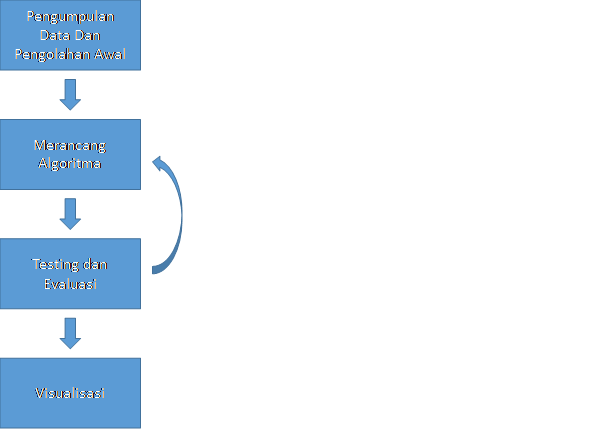
\includegraphics[scale=1]{pics/gbr3_1.png} 


%-----------------------------------------------------------------------------%
\section{Pengumpulan Data dan Pengolahan Awal}
%-----------------------------------------------------------------------------%
Data microarray tersedia secara bebas di geo [http://www.ncbi.nlm.nih.gov/geo/], dan dapat diunduh, untuk digunakan sebagai data penelitian. Kemudian dilakukan normalisasi standar yang sering di pakai pada data microarray, proses normalisasi ada banyak metode, dan akan digunakan satu metode standar untuk pengolahan awal microarray agar mendapatkan data konsisten dan dapat dibandingkan. Proses pengolahan awal dan normalisasi digunakan tools standar dan tersedia bebas yaitu R-Bioconductor. \\

\todo { ambil source dari geo2r }

%-----------------------------------------------------------------------------%
\section{Data Profil Gen Percobaan Microarray dan Biomarker}
%-----------------------------------------------------------------------------%
\todo { terangkan data profil gen sitasi pada paper : \\
1. paper tentang multi \\
2. papernya gse10072 \\
3. contoh tabel ekspresi gen \\
4. detail kondisi pasien }

%-----------------------------------------------------------------------------%
\section{Perancangan Algoritma}
%-----------------------------------------------------------------------------%
Pada penelitian ini, akan dibangun sebuah teknik pencarian \textit{Biomarker} dengan metode seleksi fitur gen. Metode ini menerapkan perankingan gen secara \textit{multi step} terhadap model yang didapatkan pada proses \textit{training}. Arsitektur yang digunakan adalah arsitektur \textit{Deep Belief Network (DBN)} yang merupakan bagian dari metode \textit{deep learning}. Metode perankingan yang digunakan adalah modifikasi dari algoritma seleksi fitur untuk \textit{logistic regression} yang dilakukan oleh \cite{shevade2003simple}. Akan tetapi metode ini memiliki masalah dalam  mengeliminasi fitur jika diterapkan secara langsung pada model DBN, dikarenakan parameter bobot (W) dan bias (b) ditempatkan disetiap fitur dan model ini hanya memiliki satu layer dibandingkan dengan DBN yang memiliki banyak layer. \\


%-----------------------------------------------------------------------------%
\subsection{Tahap Unsupervised}
%-----------------------------------------------------------------------------%
Tahap unsupervised adalah tahapan dimana model DBN ditraining secara unsupervised dengan data training pada tiap-tiap layernya secara greedy. Tiap layernya dihitung cost untuk kemudian diminimisasi errornya.

%-----------------------------------------------------------------------------%
\subsection{Tahap Supervised}
%-----------------------------------------------------------------------------%
Pada saat training unsupervised dilakukan untuk merekonstruksi xxx
oleh karena itu tidak diketahui xxx
\todo {baca dan cari referensi supervised dan unsupervised}

%-----------------------------------------------------------------------------%
\subsection{Tahap Tuning Parameter}
%-----------------------------------------------------------------------------%


%-----------------------------------------------------------------------------%
\section{Melakukan Testing Arsitektur DBN}
%-----------------------------------------------------------------------------%
\todo {buat bagan pengujian arsitektur DBN }
Hasil dari unsupervised learning yang dilakukan oleh DBN, akan diuji dahulu dengan dengan data testing, apakah error rekonstruksinya lebih baik. Setelah dilakukan perankingan biomarker, diperlukan pengujian apakah apakah seleksi fitur tersebut menggambarkan hasil yang diinginkan, dengan membandingkan biomarker yang dihasilkan dengan literature. 

%-----------------------------------------------------------------------------%
\section{Implementasi Metode Perangkingan Bobot Secara Multi Step Untuk Mendapatkan Gen Biomarker}
%-----------------------------------------------------------------------------%
\todo { insert gambar 1 pada presentasi  }
\todo { beri keterangan perhitungan dan algoritmanya}
\\

\begin{algorithm}[H]
 \KwData{this text}
 \KwResult{how to write algorithm with \LaTeX2e }
 initialization\;
 \While{not at end of this document}{
  read current\;
  \eIf{understand}{
   go to next section\;
   current section becomes this one\;
   }{
   go back to the beginning of current section\;
  }
 }
 \caption{How to write algorithms}
\end{algorithm}

\todo { beri keterangan code pythonnya  }




%-----------------------------------------------------------------------------%
\section{Evaluasi Hasil Perangkingan Dengan Klasifikasi Secara Supervised}
%-----------------------------------------------------------------------------%
Evaluasi hasil hasil perankingan secara supervised diperlukan untuk mengetahui apakah hasil perankingan tersebut memperbaiki hasil klasifikasi pasien kanker dan sehat hanya dengan menggunakan gen-gen yang dipilih berdasarkan ranking yang didapatkan.


%-----------------------------------------------------------------------------%
\section{Perbandingan Hasil Perangkingan Dengan Literatur}
%-----------------------------------------------------------------------------%

Hasil perankingan pada percobaan tersebut selanjutnya diteliti apakah gen hasil perankingan tersebut adalah gen yang memiliki signifikansi terhadap penyakit yang diinginkan. Dalam kasus ini yaitu penyakit kanker paru-paru.


